\subsection*{НГУ-2.32}

\setcounter{equation}{0}

\begin{abstract}
Заземленная проводящая плоскость имеет выступ в форме полусферы радиуса $a$. Центр полусферы лежит на плоскости. На оси симметрии системы на расстоянии $b > a$ от плоскости находится точечный заряд $q$. Найти потенциал электрического поля, а также заряд $Q$, индуцированный на выступе.
\end{abstract}

\noindent \hrulefill
\\
\begin{wrapfigure}[6]{r}{0.30\textwidth}
	\raisebox{0pt}[\dimexpr\height-2\baselineskip\relax]{
	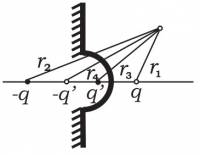
\includegraphics[width=0.30\textwidth]{pics/2.32.jpg}}
\end{wrapfigure}

Используя метод изображений: 

* Потенциал на плоскости равен $0 \rightarrow$ виртуальный заряд $(-q)$ расположен на расстоянии $b$ от плоскости.

* Потенциал на выступе равен $0 \rightarrow$ виртуальный заряд $q'=-q \times \frac{a}{b}$ расположен на расстоянии $b'=\frac{a^2}{b}$ от плоскости.

* Потенциал на плоскости равен $0 \rightarrow$ виртуальный заряд $(-q')$ расположен на расстоянии $b'$ от плоскости.

Потенциал в любой точке:

$$\phi = k \times (\frac{q}{r_1} - \frac{q}{r_2} + \frac{q'}{r_3} - \frac{q'}{r_4})$$

 Пусть $r$ - радиус, который соединяет центр выступа с любой точкой. $\theta$ - это угол, образованный симметричной линией и этим радиусом.

$$r_1 = \sqrt{b^2 + r^2 -2br \cos{\theta}}$$

$$r_2 = \sqrt{b^2 + r^2 +2br \cos{\theta}}$$

$$r_3 = \sqrt{b'^2 + r^2 -2b'r \cos{\theta}}$$

$$r_4 = \sqrt{b'^2 + r^2 +2b'r \cos{\theta}}$$

Напряжение в любой точке:

$$E = -\frac{\partial\phi}{\partial r}$$

Напряжение в точке, которая лежит на поверхности выступа (Заменим $r = a$ и сократим процесс преобразования:):

$$E = q \times \frac{b^2-a^2}{4 \pi a} \times [\frac{1}{(b^2+a^2+2ab\cos{\theta})^\frac{3}{2}}  - \frac{1}{(b^2+a^2-2ab\cos{\theta})^\frac{3}{2}}]$$

Плотность заряда, распределенного на поверхности выступа, равна $\sigma$. Применяя закон Гаусса:

$$E = \frac{\sigma}{\epsilon_0} \rightarrow \sigma = E \times \epsilon_0$$

Заряд на поверхности выступа равен:

$$Q = \displaystyle \int \sigma \times dS = \displaystyle \int_{0}^{\pi/2} \sigma \times (2 \pi a \sin{\theta})(a \times d\theta) = -q \times (1-\frac{b^2-a^2}{b \sqrt{b^2+a^2}})$$

\textbf{Ответ:}

$$Q =  -q \times (1-\frac{b^2-a^2}{b \sqrt{b^2+a^2}}).$$






